\documentclass[UTF8,a4paper]{article}% 文档格式
\usepackage{graphicx}
\usepackage{physics}
\usepackage{ctex}
\usepackage{times}% 英文使用Times New Roman
\usepackage[left=1cm,right=1cm,top=1.80cm,bottom=1.8cm]{geometry}
\usepackage{fancyhdr}
\pagestyle{fancy}
\usepackage{multirow}
\usepackage{siunitx}
\usepackage{float}

\title{\textbf{基础物理实验报告\\偏振光学系列}}
\author{杨哲涵~~~工物22班~~~2022011105}
\date{2023年11月16日}
\begin{document}
\maketitle
\lhead{2023年基础物理学实验A2}
\chead{}
\rhead{42a}
\lfoot{}
\cfoot{\thepage}
\rfoot{}
\section*{摘要}
本实验利用半导体激光器与光强探测器测试了布儒斯特角和偏振器的特性,并观察了1/4波片,1/2波片的性质.依靠上述实验数据测定了椭圆偏振光的相关参数.
\section{实验原理与仪器}
\paragraph{实验原理}
由Maxwell的电磁理论,我们已知道光是一种电磁波.我们一般用光波的电矢量(光矢量)的振动状态来描述光波的偏振.
\subparagraph{光的偏振态}
按光矢量的振动状态可把光波偏振态大体分成五种:自然光,部分偏振光,椭圆偏振光,圆偏振光和线偏振光.一个单色偏振光可分解为两个偏振方向互相垂直的线偏振光的叠加:
\begin{align*}
    E_x & =a_1\cos(\omega t)        \\
    E_y & =a_2\cos(\omega t+\delta)
\end{align*}
取$\alpha=\arctan(\frac{a_2}{a_1}\cos\delta)$为偏振方向与$x$轴的夹角.当$\delta=0,\pi$时,对应线偏振光.当$\delta=\pi/2,-\pi/2$且$a_1=a_2$时,为圆偏振光.其他情况都对应椭圆偏振光.

定义辅助角$\beta=\arctan(\frac{a_2}{a_1})$,$\Psi$为长轴方位角,$a,b$为长半轴与短半轴.
\begin{align*}
    \psi            & =\frac{1}{2}\arctan(\tan2\beta\cos\delta)        \\
    \frac{b^2}{a^2} & =\frac{2}{1+\sqrt{1-(\sin\delta\sin2\beta)^2}}-1
\end{align*}
\subparagraph{偏振片}
偏振片有一个透射轴和一个与之垂直的消光轴,对于理想的偏振片,只有电矢量振动方向与透射轴方向平行的光波分量才能通过偏振片.

实际的偏振片有主透射率和消光比两个主要性能指标.沿透射轴方向振动的光波的光强透射率为$T_1$,沿消光轴方向振动的光波的光强透射率为$T_2$.主透射率之比$T_2/T_1$记为消光比$e$.

\subparagraph{反射与折射的起偏现象}
从空气到介质表面的反射,投射率分别为
\begin{align*}
    R_p & =r_p^2=\left(\frac{\tan(\theta_i-\theta_t)}{\tan(\theta_i+\theta_t)}\right)^2 \\
    T_p & =1-R_p                                                                        \\
    R_s & =r_s^2=\left(\frac{\sin(\theta_i-\theta_t)}{\sin(\theta_i+\theta_t)}\right)^2 \\
    T_s & =1-R_s
\end{align*}
从中可知,当$\theta_i+\theta_t=\frac{\pi}{2}$时,反射光中电矢量都不在入射面内,这个特征入射角$\theta_i=\arctan n=\theta_B$称为布儒斯特角.
\subparagraph{延迟器与波片}
常用的线性延迟器是由双折射材料制成的光学元件,一对沿特定方向振动的同频正交线偏振光经过延迟器后偏振态保持不变,但因两偏振光分量传播速度不同而使较慢的分量相比另一分量相位延迟了$\delta_r$,前者记为慢轴,后者记为快轴.

$\delta_r=N\pi\pm\pi/2$的延迟器称为1/4波片.$\delta_r$为$\pi$奇数倍的称为1/2波片.$\delta_r$为$\pi$偶数倍的称为全波片.
\subparagraph{椭圆偏振光的长轴方位角$\psi$和波片相延$\delta_r$}
在本实验中,我们用$\psi$和$\frac{b^2}{a^2}$两个量来描述椭圆偏振光的偏振态.可用检偏器和光强探测器来分析.对于理想的检偏器,其透射轴平行于椭圆长轴时透射光强正比于$a^2$,为极大值.透射轴平行于椭圆短轴时透射光强正比于$b^2$,为极小值 .旋转检偏器的透射轴的方向,就可以用光强探测器示值确定出椭圆长轴方位角$\psi$和光强的极值比.

多数情况下近似有$\frac{b^2}{a^2}=I_{min}/I_{max}$以及
$$|\sin\delta_r|=\frac{2\sqrt{I_{min}/I_{max}}}{(\sin2\beta)(1+I_{min}/I_{max})}$$
\paragraph{实验仪器}
本实验用到以下仪器
\begin{itemize}
    \item 波长为650$\unit{\nm}$的半导体激光器
    \item 起偏器P和检偏器A
    \item 两个1/4波片$C_0$,$C_x$
    \item 光强探测器,由硅光电池,数字电压表与电阻箱组成
\end{itemize}
\section{实验内容}
\subsection*{A 准备工作}
开启激光电源,确认激光束由光源发出通过起偏管偏振片,由检偏管偏振片射出,一般情况下这里不需要调节.利用反射元件调整小平台与分光计主光轴基本垂直,通常平台的初始位置已经垂直.
\subsection*{B 观察布儒斯特角和偏振器特性}
\paragraph{观察布儒斯特角}
按照说明调节反射元件后,在入射角约为$\ang{56}$的情况下观察到反射光点最暗,此时注意到经过偏振器P的光相当明亮,说明正确找到了布儒斯特角.
\begin{table}[H]
    \caption{观察布儒斯特角}
    \centering
    \begin{tabular}{cccc}
        \hline
        \multicolumn{4}{l}{正入射时平台方位角$\alpha_{i=0}=\ang{306;30}$}                          \\ \hline
          & 平台方位角$\alpha_B$ & 布儒斯特角的测量值$\theta_B$ & 起偏器P的透射轴在水平方向的夹角$p_{\leftrightarrow}$ \\ \hline
        1 & \ang{249;25}    & \ang{57;5}          & \ang{270.1}                           \\
        2 & \ang{249;26}    & \ang{57;4}          & \ang{270.0}                           \\
        3 & \ang{249;25}    & \ang{57;5}          & \ang{270.1}                           \\ \hline
    \end{tabular}
\end{table}
计算得到平均$\theta_B=$\ang{57;4.67},折射率 $n=1.544$.实验中由于表面散射等原因,测定布儒斯特角的准确度较低.
\paragraph{确定偏振器透射轴方向}
由上面的数据可计算出P的透射轴在水平方向的夹角的平均值为$\ang{270.067}$.

移去反射元件,转动检偏器A使A和P正交消光(利用光强探测器判断),此时记录下A盘的刻度度数为$a_\updownarrow=\ang{4}$.
\paragraph{测量透射轴夹角}
取两个偏振器的若干不同组透射轴夹角测量透射光强为:
\begin{table}[H]
    \centering
    \caption{透射光强$I_m$与两偏振器夹角$\theta$的关系}
    \begin{tabular}{l|llllllllll}
        \hline
        夹角$\theta$                & \ang{0}  & \ang{15}  & \ang{30}  & \ang{45}  & \ang{60}  & \ang{75}  & \ang{80}  & \ang{84}  & \ang{87}  & \ang{90}  \\
        $a=a_\updownarrow+\theta$ & \ang{94} & \ang{109} & \ang{124} & \ang{139} & \ang{154} & \ang{169} & \ang{174} & \ang{178} & \ang{181} & \ang{184} \\
        $I_m(\unit{\mV})$         & 7.211    & 6.681     & 5.300     & 3.475     & 1.699     & 0.433     & 0.185     & 0.086     & 0.013     & 0.009     \\
        相对$\cos^2\theta$偏差        & 0.00\%   & -0.71\%   & -2.05\%   & -3.75\%   & -6.14\%   & -12.11\%  & -18.96\%  & -2.15\%   & -79.72\%  & 0.00\%    \\\hline
    \end{tabular}
\end{table}
略微处理数据,可以绘出$\lambda=(I_m-I_{min})/(I_{max}-I_{min})$与$\cos^2\theta$随$\theta$的变化情况,两者的趋势符合得很好,这验证了马吕斯定律.
\begin{figure}[H]
    \centering
    \begin{minipage}[t]{0.5\linewidth}
        \centering
        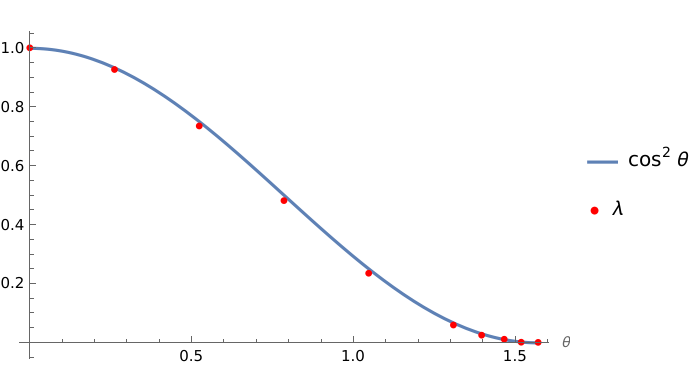
\includegraphics[width=0.9\linewidth]{marius-law.png}
        \caption{$\lambda$与$\cos^2\theta$随$\theta$的变化情况}
        \label{fg:marius}
    \end{minipage}
\end{figure}
可以注意到$\lambda$相较$\cos^2\theta$略微偏小,这是因为还有环境光进入光强探测器,使得接收到的光并非全部来自两个偏振器.
\subsection*{C 波片的特性研究}
\paragraph{定波片方向}
波片$C_0$快轴在竖直方向与波片$C_x$某轴在竖直方向的实验结果如下:
\begin{table}[H]
    \centering
    \caption{定波片$C_0$与$C_x$的快轴的方向}
    \begin{tabular}{lll}
        \hline
        $R$            & $p=p_\leftrightarrow$ & $a=a_\updownarrow$ \\
        100\unit{\ohm} & \ang{270.067}         & \ang{4}            \\ \hline
        \multicolumn{3}{c}{$C_0=\ang{77.1}$}                        \\ \hline
    \end{tabular}
    \begin{tabular}{lll}
        \hline
        $R$            & $p=p_\leftrightarrow$ & $a=a_\updownarrow$ \\
        100\unit{\ohm} & \ang{270.067}         & \ang{4}            \\ \hline
        \multicolumn{3}{c}{$C_x=\ang{80.0}$}                        \\ \hline
    \end{tabular}
\end{table}
\paragraph{观测偏振光通过1/2波片或全波片的现象}
注意到,如果两个偏振器的快轴重合,那么偏振光通过了一个1/2波片,如果一者快轴与一者慢轴重合,那么偏振光通过了一个全波片.
\begin{table}[H]
    \centering
    \caption{观测偏振光通过1/2波片或全波片的现象}
    \begin{tabular}{llll}
        \cline{2-4}
                                    & \multicolumn{3}{c}{$C_x=\ang{80}$某轴竖直,$C_0=\ang{77.1}$快轴竖直}                             \\ \hline
        $\beta=p-p_\leftrightarrow$ & \ang{15}                                                    & \ang{30}    & \ang{45}    \\
        $p$                         & \ang{285.4}                                                 & \ang{300.4} & \ang{356.4} \\
        消光$a_i$                     & \ang{17.3}                                                  & \ang{32.3}  & \ang{48.2}  \\
        $\alpha=a_i-a_\updownarrow$ & \ang{13.3}                                                  & \ang{28.3}  & \ang{44.3}  \\\hline
    \end{tabular}
    \begin{tabular}{lll}
        \hline
        \multicolumn{3}{c}{$C_x=\ang{80}$某轴竖直,$C_0=\ang{167.1}$快轴水平} \\
        \hline
        \ang{15}    & \ang{30}    & \ang{45}                         \\
        \ang{285.4} & \ang{300.4} & \ang{356.4}                      \\
        \ang{349.0} & \ang{334.0} & \ang{319.0}                      \\                    \ang{-15.0}                                        &    \ang{-30.0}         &     \ang{-45.0}        \\\hline
    \end{tabular}
\end{table}
实验中两个圆盘是相对摆放的,刻度读取的方式一样.如果$\beta=-\alpha$,说明偏振光经过后没有受到改变,如果$\beta=\alpha$说明偏振光旋转了$\beta$.

因此从表中可以看出,$C_x=\ang{80}$的慢轴是竖直的.
\paragraph{线偏振光通过1/4波片}
分别用 $\psi=\ang{90}-\alpha$与前述原理部分公式计算得到如下结果:
\begin{table}[H]
    \centering
    \caption{线偏振光通过1/4波片}
    \begin{tabular}{llll}
        \hline
        \multicolumn{2}{c}{$C_0=\ang{77.1}$}            & $R=100\unit{\ohm} $ & $I_0=0.03\unit{\mV}$               \\
        \hline
        $\beta=p-p_\leftrightarrow$                     & \ang{22.5}          & \ang{45.0}           & \ang{67.5}  \\
        $p$                                             & \ang{292.5}         & \ang{315.0}          & \ang{337.5} \\
        $a_i$                                           & \ang{91}            & \ang{44.4}           & \ang{3.0}   \\
        $I_{max}(\unit{\mV})$                           & 5.258               & 3.205                & 2.703       \\
        $I_{min}(\unit{\mV})$                           & 0.926               & 2.955                & 0.600       \\
        $\alpha=a_i-a_\updownarrow$                     & \ang{87.0}          & \ang{40.4}           & \ang{-1.0}  \\
        利用$\alpha$计算$\psi$                              & \ang{3.0}           & \ang{49.6}           & \ang{91.0}  \\
        $\frac{b^2}{a^2}\approx\frac{I_{min}}{I_{max}}$ & 0.176               & 0.921                & 0.222       \\
        $|\sin\delta_r|$                                & 0.9996              & 0.9695               & 1.0310      \\
        $\delta_r$                                      & \ang{88.40}         & \ang{75.81}          &             \\
        利用$\delta_r$计算$\psi$                            & \ang{1.59}          & \ang{90.00}          &             \\
        \hline
    \end{tabular}
\end{table}
\section{讨论}
观察偏振光通过1/4波片时,计算中遇到了$\psi=\ang{90}$,这是因为在$\beta=\arctan(\frac{a_2}{a_1})=\ang{45}$时,情况退化为圆偏振光,对于圆偏振光,无法指出其长轴的方位轴,反应在公式里,有$\tan2\beta \cdot\cos\delta=\infty$. 这是个病态的等式,因此根据$\psi=\frac{1}{2}\arctan(\tan2\beta\cos\delta)$计算出来的值始终是$\ang{90}$,不再反应真实的长轴方位轴.


并且,从$\beta=\ang{45}$的数据中可以看到,光强探测器精度与其他因素对$\frac{b^2}{a^2}$造成的损失近似为$10\%$,使得在$\beta=\ang{67.5}$处也遇到了无法处理的情况,不能利用公式计算$\delta_r$.
\appendix
\section{附录}
\begin{figure}[H]
    \centering
    \begin{minipage}[t]{0.9\linewidth}
        \centering
        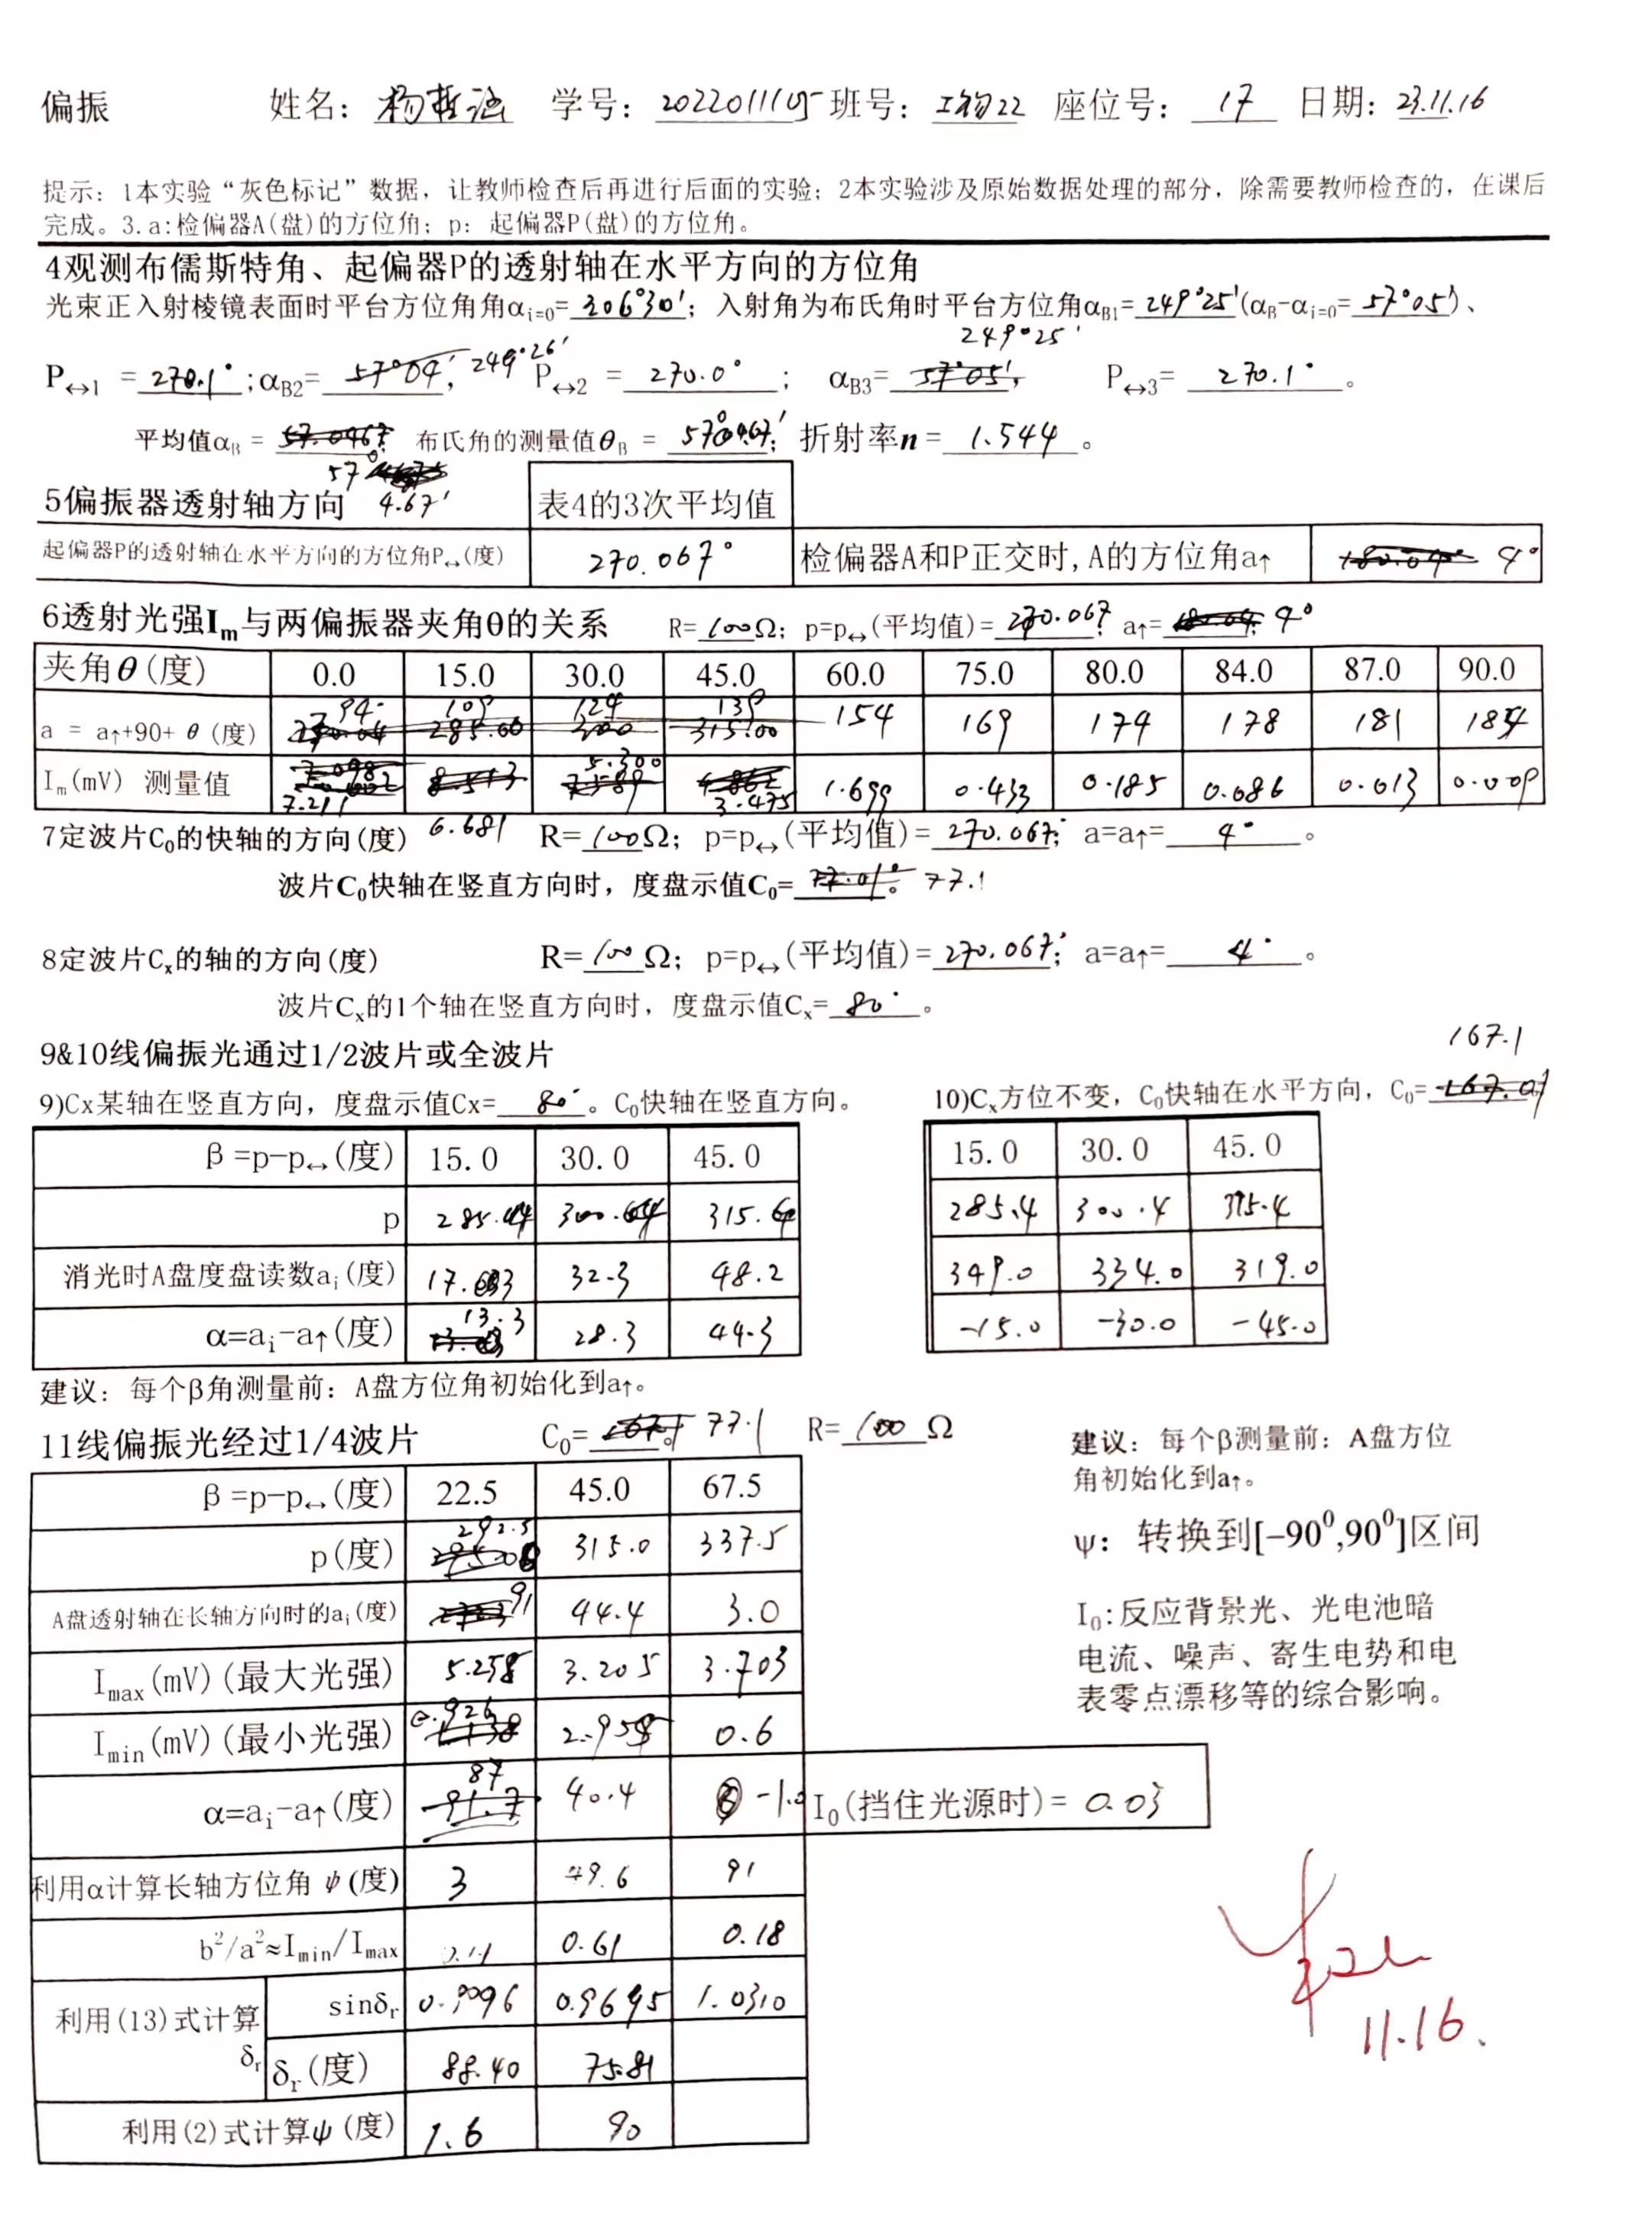
\includegraphics[width=0.9\linewidth]{data.jpeg}
        \caption{原始数据}
    \end{minipage}
\end{figure}
\end{document}
\end{document}